\documentclass[rep.tex]{subfiles}
\begin{document}

\chapter{Zadanie 3}
\label{zad3}
\section{Treść}
Zaprojektować powietrzną linię cylindryczno–płaską o przekroju poprzecznym jak na rys.~\ref{fig:zad3:line} zakładając,
że jej impedancja charakterystyczna jest równa $Z_0 = 30~\Omega$.
Odległość pomiędzy równoległymi przewodzącymi płaszczyznami tej linii jest równa~$b = 9~mm$.
O ile zmieni się impedancja charakterystyczna tej linii (zaprojektowanej) po wypełnieniu jej
bezstratnym dielektrykiem o~$\epsilon_r = 2.04$ i $\mu_r = 1$.

\begin{figure}[!htbp]
  \centering
  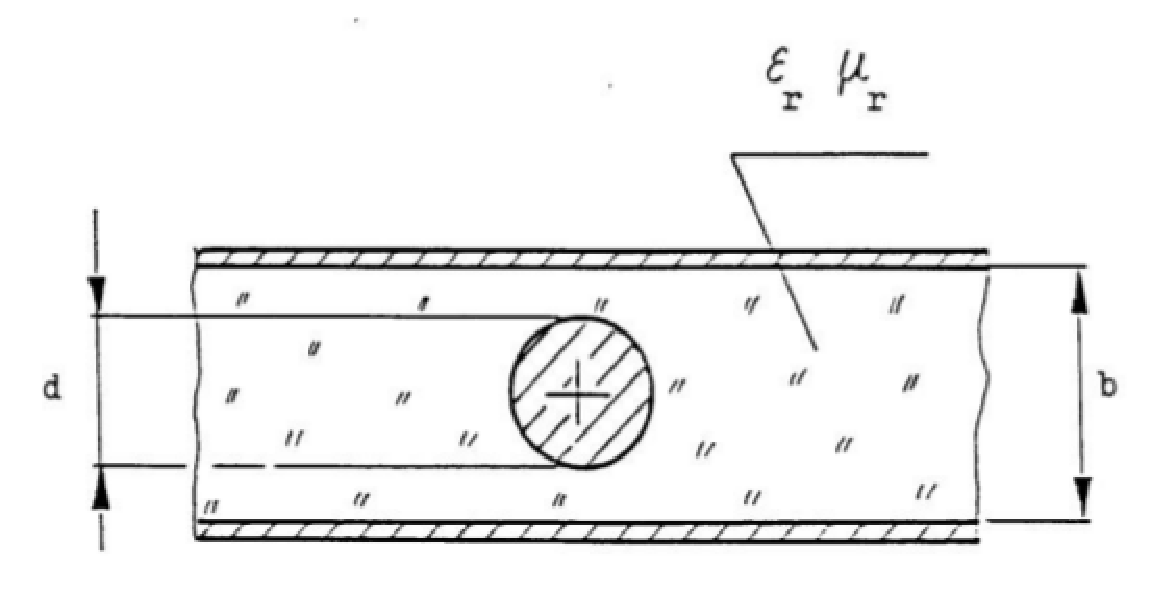
\includegraphics[scale=0.5]{fig/zad3/line}
  \caption{Linia cylindryczno-płaska}
  \label{fig:zad3:line}
\end{figure}

\section{Rozwiązanie}
Impedancja charakterystyczna linii cylindryczno-płaskiej wyraża się wzorem:
\begin{equation}
  Z_0\Big(\frac{d}{b}\Big) = 59.952 \sqrt{\frac{\mu_r}{\epsilon_r}} \Big(\ln{\frac{\sqrt{x} + \sqrt{y}}{\sqrt{x - y}}} - \frac{R^4}{30} + 0.014R^8\Big),
  \label{eqn:zad3:z}
\end{equation}
gdzie:
\begin{align}
  R &= \frac{\pi}{4} \frac{d}{b} \\
  x &= 1 + 2\operatorname{sh}^2\,(R) \\
  y &= 1 - 2\sin^2(R)
\end{align}

Zależność impedancji od wymiarów linii jest znacznie bardziej złożona niż w przypadku linii z zadania~\ref{zad2}.
Dlatego w tym przypadku nie można znaleźć rozwiązania w sposób analityczny.
W celu określenia wymiarów linii należy rozwiązać równanie:
\begin{equation}
  Z_0\Big(\frac{d}{b}\Big)\Big\arrowvert_{d=9~mm} - 30 \Omega = 0
  \label{eqn:zad3:eq}
\end{equation}
Do znalezienia rozwiązania użyto zaprogramowanego poprzednio algorytmu Newtona-Raphsona.

Otrzymano następujące wyniki:
\begin{align}
  d   &= 6.73875214859~mm \\
  Z_0 &= 30.0~\Omega
\end{align}

W celu odpowiedzi na drugie pytanie należy policzyć impedancje linii korzystając ze wzoru~\ref{eqn:zad3:z}.
Jednak zamiast $\mu_r = 1$ i $\epsilon_r = 1$, podstawić wartości określone w treści zadania.
Uzyskana w ten sposób wartość impedancji wynosi $Z_0 = 21.0042012604~\Omega$.
Zmieni się ona zatem o $-8.99579873958~\Omega$.

Zmiana impedancji wynika też bezpośrednio ze wzoru~\ref{eqn:zad3:z}.
Po wstawieniu dielektryka nowa wartość impedancji wyniesie~$Z_0 \times \sqrt{\mu_r}$.
\end{document}
